 \providecommand{\main}{../..}
\documentclass[\main/main.tex]{subfiles}
\begin{document}
\subsection{Esercizio 2.7}

\begin{figure}
  \begin{align*}
    \max z = 2x_1 + x_2  \\
    x_1 + x_2   & \leq 1 \\
    9x_1 + 3x_2 & \leq 6 \\
    3x_1 + 2x_2 & \geq 1 \\
    x_1, x_2    & \geq 0
  \end{align*}
  \caption{Esercizio 2.7}
\end{figure}

\subsection{Risoluzione esercizio 2.7}

\begin{figure}
  \begin{subfigure}{0.45\textwidth}
    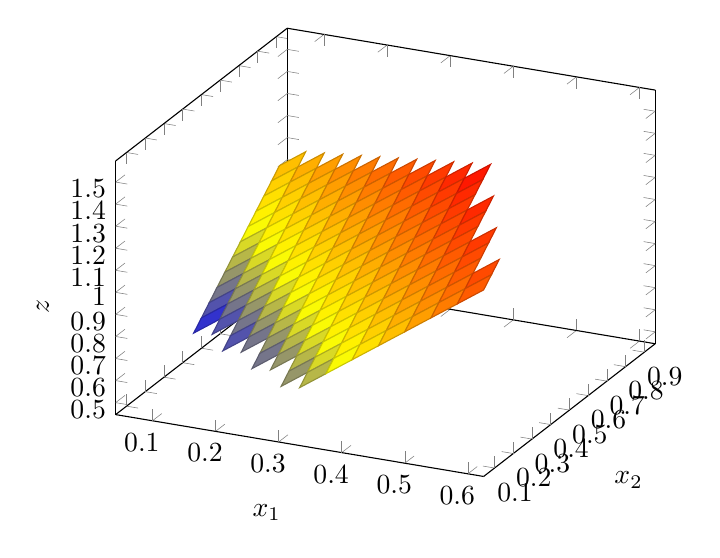
\begin{tikzpicture}
      \begin{axis}[
          xlabel=$x_1$,
          ylabel=$x_2$,
          zlabel=$z$,
          domain=0:1,
          y domain= 0:1,
          ytick = {0,0.1,...,1},
          xtick = {0,0.1,...,1},
          ztick = {0,0.1,...,2}
        ]
        \addplot3[surf, unbounded coords=jump]
        {
          x + y < 1 &&
          9*x+3*y < 6 &&
          3*x + 2*y > 1 &&
          x > 0 &&
          y > 0?
          2*x+y:NaN
        };
      \end{axis}
    \end{tikzpicture}
    \caption{La funzione $z$}
  \end{subfigure}
  ~
  \begin{subfigure}{0.45\textwidth}
    \includegraphics[width=0.8\textwidth]{2_7}
    \caption{I vincoli del problema nello spazio $x_1 - x_2$}
  \end{subfigure}
  \caption{Risoluzione esercizio 2.7}
\end{figure}



\end{document}